%%%%%%%%%%%%%%%%%%%%%%%%%%%%%%%%%%%%%%%%%
% Programming/Coding Assignment
% LaTeX Template
%
% This template has been downloaded from:
% http://www.latextemplates.com
%
% Original author:
% Ted Pavlic (http://www.tedpavlic.com)
%
% Note:
% The \lipsum[#] commands throughout this template generate dummy text
% to fill the template out. These commands should all be removed when 
% writing assignment content.
%
% This template uses a Perl script as an example snippet of code, most other
% languages are also usable. Configure them in the "CODE INCLUSION 
% CONFIGURATION" section.
%
%%%%%%%%%%%%%%%%%%%%%%%%%%%%%%%%%%%%%%%%%

%----------------------------------------------------------------------------------------
%	PACKAGES AND OTHER DOCUMENT CONFIGURATIONS
%----------------------------------------------------------------------------------------

\documentclass{article}

\usepackage{fancyhdr} % Required for custom headers
\usepackage{lastpage} % Required to determine the last page for the footer
\usepackage{extramarks} % Required for headers and footers
\usepackage[usenames,dvipsnames]{color} % Required for custom colors
\usepackage{graphicx} % Required to insert images
\usepackage{subcaption}
\usepackage{listings} % Required for insertion of code
\usepackage{courier} % Required for the courier font
\usepackage{lipsum} % Used for inserting dummy 'Lorem ipsum' text into the template
\usepackage{amsfonts}
\usepackage{amssymb}
\usepackage{amsmath}
\usepackage{enumerate}
\usepackage{soul}
%Code for including Python code in Latex - outlined on the Piazza forum post, taken from Stackoverflow

\usepackage{enumitem}
\usepackage[utf8]{inputenc}
\definecolor{dkgreen}{rgb}{0,0.6,0}
\definecolor{gray}{rgb}{0.5,0.5,0.5}
\definecolor{mauve}{rgb}{0.58,0,0.82}

\lstset{frame=tb,
  language=Python,
  aboveskip=3mm,
  belowskip=3mm,
  showstringspaces=false,
  columns=flexible,
  basicstyle={\small\ttfamily},
  numbers=none,
  numberstyle=\tiny\color{gray},
  keywordstyle=\color{blue},
  commentstyle=\color{dkgreen},
  stringstyle=true{mauve},
  breaklines=true,
  breakatwhitespace=true,
  tabsize=3
}

% Margins
\topmargin=-0.45in
\evensidemargin=0in
\oddsidemargin=0in
\textwidth=6.5in
\textheight=9.0in
\headsep=0.25in

% Paragraph spacing
\setlength{\parskip}{10pt}


\linespread{1.1} % Line spacing

% Set up the header and footer
\pagestyle{fancy}
\lhead{\hmwkAuthorName} % Top left header
\chead{\hmwkClass\ (\hmwkClassTime): \hmwkTitle} % Top center head
%\rhead{\firstxmark} % Top right header
\lfoot{\lastxmark} % Bottom left footer
\cfoot{} % Bottom center footer
\rfoot{Page\ \thepage\ of\ \protect\pageref{LastPage}} % Bottom right footer

\setlength\parindent{0pt} % Removes all indentation from paragraphs

%----------------------------------------------------------------------------------------
%	CODE INCLUSION CONFIGURATION
%----------------------------------------------------------------------------------------

\definecolor{MyDarkGreen}{rgb}{0.0,0.4,0.0} % This is the color used for comments
\lstloadlanguages{Perl} % Load Perl syntax for listings, for a list of other languages supported see: ftp://ftp.tex.ac.uk/tex-archive/macros/latex/contrib/listings/listings.pdf
\lstset{language=Perl, % Use Perl in this example
        frame=single, % Single frame around code
        basicstyle=\small\ttfamily, % Use small true type font
        keywordstyle=[1]\color{Blue}\bf, % Perl functions bold and blue
        keywordstyle=[2]\color{Purple}, % Perl function arguments purple
        keywordstyle=[3]\color{Blue}\underbar, % Custom functions underlined and blue
        identifierstyle=, % Nothing special about identifiers                                         
        commentstyle=\usefont{T1}{pcr}{m}{sl}\color{MyDarkGreen}\small, % Comments small dark green courier font
        stringstyle=\color{Purple}, % Strings are purple
        showstringspaces=false, % Don't put marks in string spaces
        tabsize=5, % 5 spaces per tab
        %
        % Put standard Perl functions not included in the default language here
        morekeywords={rand},
        %
        % Put Perl function parameters here
        morekeywords=[2]{on, off, interp},
        %
        % Put user defined functions here
        morekeywords=[3]{test},
       	%
        morecomment=[l][\color{Blue}]{...}, % Line continuation (...) like blue comment
        numbers=left, % Line numbers on left
        firstnumber=1, % Line numbers start with line 1
        numberstyle=\tiny\color{Blue}, % Line numbers are blue and small
        stepnumber=5 % Line numbers go in steps of 5
}

% Creates a new command to include a perl script, the first parameter is the filename of the script (without .pl), the second parameter is the caption
\newcommand{\perlscript}[2]{
\begin{itemize}
\item[]\lstinputlisting[caption=#2,label=#1]{#1.pl}
\end{itemize}
}

%----------------------------------------------------------------------------------------
%	DOCUMENT STRUCTURE COMMANDS
%	Skip this unless you know what you're doing
%----------------------------------------------------------------------------------------

% Header and footer for when a page split occurs within a problem environment
\newcommand{\enterProblemHeader}[1]{
%\nobreak\extramarks{#1}{#1 continued on next page\ldots}\nobreak
%\nobreak\extramarks{#1 (continued)}{#1 continued on next page\ldots}\nobreak
}

% Header and footer for when a page split occurs between problem environments
\newcommand{\exitProblemHeader}[1]{
%\nobreak\extramarks{#1 (continued)}{#1 continued on next page\ldots}\nobreak
%\nobreak\extramarks{#1}{}\nobreak
}

\setcounter{secnumdepth}{0} % Removes default section numbers
\newcounter{homeworkProblemCounter} % Creates a counter to keep track of the number of problems
\setcounter{homeworkProblemCounter}{-1}

\newcommand{\homeworkProblemName}{}
\newenvironment{homeworkProblem}[1][Problem \arabic{homeworkProblemCounter}]{ % Makes a new environment called homeworkProblem which takes 1 argument (custom name) but the default is "Problem #"
\stepcounter{homeworkProblemCounter} % Increase counter for number of problems
\renewcommand{\homeworkProblemName}{#1} % Assign \homeworkProblemName the name of the problem
\section{\homeworkProblemName} % Make a section in the document with the custom problem count
\enterProblemHeader{\homeworkProblemName} % Header and footer within the environment
}{
\exitProblemHeader{\homeworkProblemName} % Header and footer after the environment
}

\newcommand{\problemAnswer}[1]{ % Defines the problem answer command with the content as the only argument
\noindent\framebox[\columnwidth][c]{\begin{minipage}{0.98\columnwidth}#1\end{minipage}} % Makes the box around the problem answer and puts the content inside
}

\newcommand{\homeworkSectionName}{}
\newenvironment{homeworkSection}[1]{ % New environment for sections within homework problems, takes 1 argument - the name of the section
\renewcommand{\homeworkSectionName}{#1} % Assign \homeworkSectionName to the name of the section from the environment argument
\subsection{\homeworkSectionName} % Make a subsection with the custom name of the subsection
\enterProblemHeader{\homeworkProblemName\ [\homeworkSectionName]} % Header and footer within the environment
}{
\enterProblemHeader{\homeworkProblemName} % Header and footer after the environment
}

%----------------------------------------------------------------------------------------
%	NAME AND CLASS SECTION
%----------------------------------------------------------------------------------------

\newcommand{\hmwkTitle}{Assignment 1} % Assignment title
\newcommand{\hmwkDueDate}{Monday,\ January\ 29,\ 2018} % Due date
\newcommand{\hmwkClass}{CSC2515} % Course/class
\newcommand{\hmwkClassTime}{L0101} % Class/lecture time
\newcommand{\hmwkAuthorName}{Matthew Wong} % Your name

%----------------------------------------------------------------------------------------
%	TITLE PAGE
%----------------------------------------------------------------------------------------

\title{
\vspace{2in}
\textmd{\textbf{\hmwkClass:\ \hmwkTitle}}\\
\normalsize\vspace{0.1in}\small{Due\ on\ \hmwkDueDate}\\
\vspace{0.1in}
\vspace{3in}
}

\author{\textbf{\hmwkAuthorName}}
%\date{} % Insert date here if you want it to appear below your name

%----------------------------------------------------------------------------------------

\begin{document}

\maketitle
\clearpage
%----------------------------------------------------------------------------------------
%	Introduction
%----------------------------------------------------------------------------------------

\begin{homeworkProblem}

\noindent \textit{Introductory information and readme instructions}

Attached, you will find the required submissions \textit{faces.py, faces.tex \& faces.pdf} in addition to the various folders of uncropped and cropped images.  Comments about the code are located in the \textit{faces.py} file and the code is separated out by function and can be run as necessary from a command line argument.  Outside of the function definitions for data retrieval, cleansing and storage, code for each section is labelled appropriately and can be run without internal dependencies.  Code was written in Python 3.5 - the packages used are outlined at the beginning of the file.

\textbf{Additional Information}:  Due to time limitations, I was unable to put all of the cropped/uncropped folders into separate directories - instead, you will find these directories with a number appended (in most cases to highlight which question was attempted).  For compilation purposes, the images that are saved as a result of code exeuction must be included in the same directory as the .tex file.


\end{homeworkProblem}
\clearpage
%----------------------------------------------------------------------------------------
%	PROBLEM 1
%----------------------------------------------------------------------------------------

% To have just one problem per page, simply put a \clearpage after each problem

\begin{homeworkProblem}

\noindent \textit{Dataset description}

The uncropped dataset contains approximately 1500 images of 12 actors and actresses of varying shapes, sizes and colours.  The various cropped dataset folders contain cropped $32 \times 32$, greyscale images that are relevant to that part outlined in the assignment specification.  The cropped images were obtained by crawling through the FaceScrub dataset and applying the bounding boxes located those files.  Overall, they seem to be accurate.  There are numerous objectives in this assignment that pertain to this dataset - but in particular, the objective was the development of a linear regression classifier using Gradient Descent to distinguish between males and females as well as categorizing individual actors and actresses.  The main data source to accomplish this task will be the greyscale pixel intensities of the cropped images.  A few of the uncropped and cropped images of various actors will be shown below.
\begin{center}
\begin{figure}[!ht]\centering
\begin{subfigure}{.3\textwidth}\centering
  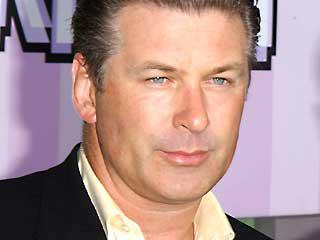
\includegraphics[width=.3\linewidth]{raw_baldwin2.jpg}
  \caption{Baldwin}
\end{subfigure}
\begin{subfigure}{.3\textwidth}\centering
  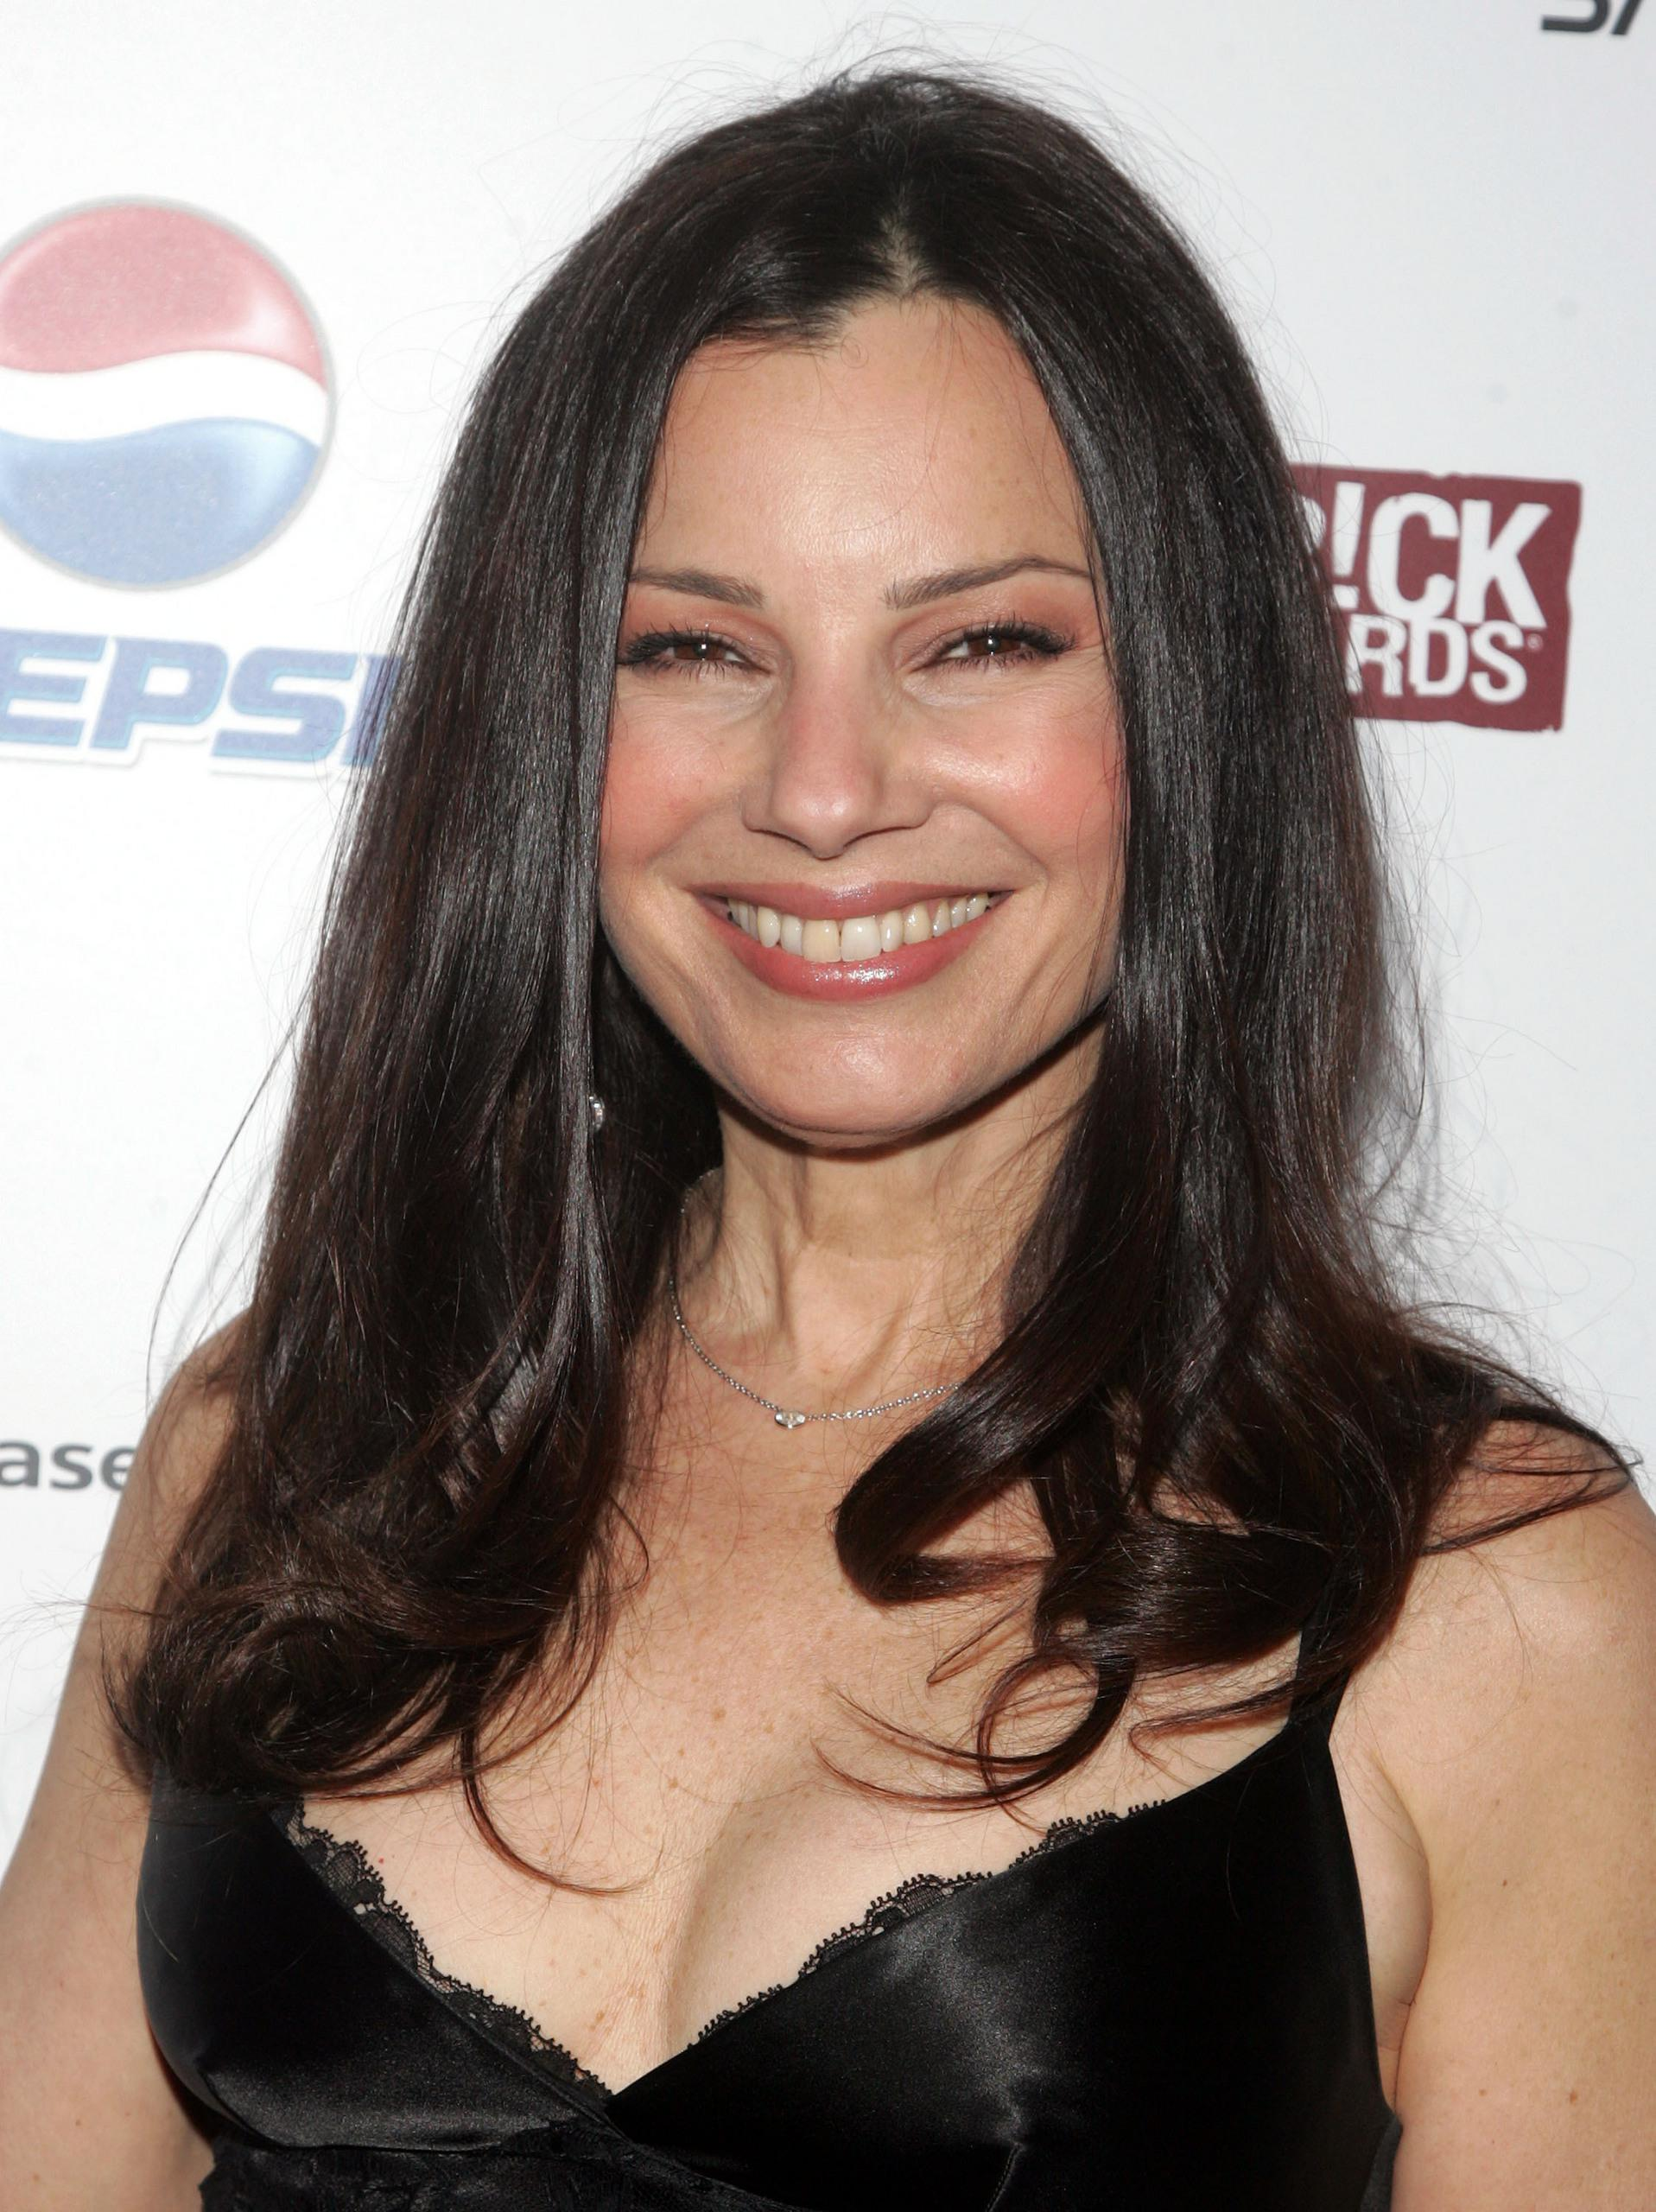
\includegraphics[width=.3\linewidth]{raw_drescher0.jpg}
  \caption{Drescher}
\end{subfigure}
\begin{subfigure}{.3\textwidth}\centering
  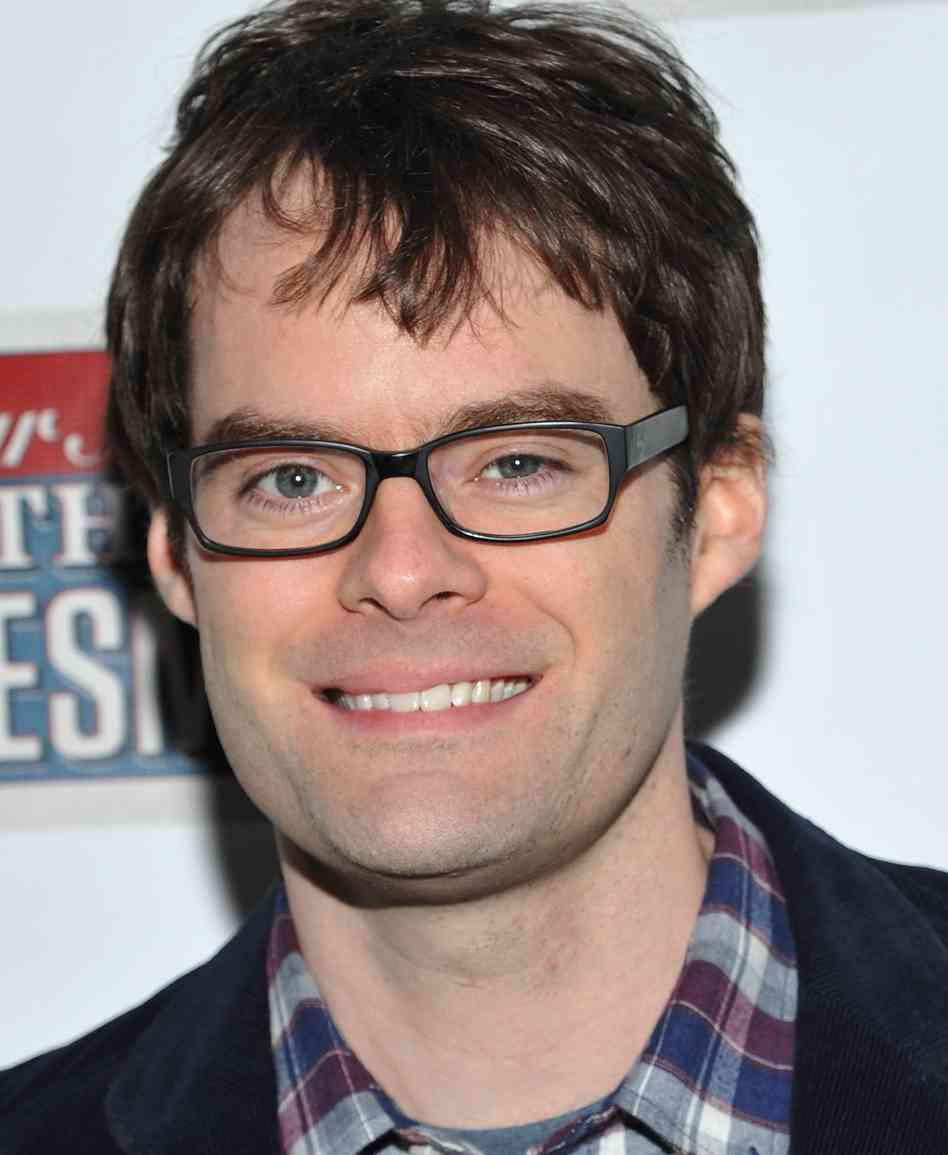
\includegraphics[width=.3\linewidth]{raw_hader0.jpg}
  \caption{Hader}
\end{subfigure}
\begin{subfigure}{.3\textwidth}\centering
  
\includegraphics[width=.3\linewidth]{baldwin2.jpg}
  \caption{Cropped Baldwin}
\end{subfigure}
\begin{subfigure}{.3\textwidth}\centering
  
\includegraphics[width=.3\linewidth]{drescher0.jpg}
  \caption{Cropped Drescher}
\end{subfigure}
\begin{subfigure}{.3\textwidth}\centering
  
\includegraphics[width=.3\linewidth]{hader0.jpg}
  \caption{Cropped Hader}
\end{subfigure}
\caption{Cropped and Uncropped sample images}
\end{figure}
\end{center}
Based on additional images from the dataset, it can stated that some actors' and actresses' faces are sometimes not directly facing the camera - hence, a superposition of the images for each actor may not be representative of their face.  Furthermore, a linear regression classifier may not be the best use case here - a logistic regression or the implementation of a convolution neural network would be more appropriate to handle rotated actors' and actresses' faces.

\end{homeworkProblem}
\clearpage
%----------------------------------------------------------------------------------------
%	PROBLEM 2
%----------------------------------------------------------------------------------------

\begin{homeworkProblem}
\noindent \textit{Splitting up the Data.}

\par The algorithm that was used to shuffle the dataset originated from the \textit{numpy.random} library.  The \textit{random.seed()} command was used and different seeds set in order to get the best results for training and validation in addition to allowing for reproducible results.  A detailed explanation of this command can be located on the official Numpy documentation.

For parts 3, 4, and 5, the data was flattened into rows of 1024 pixels.  The label (either Carell vs.  Baldwin or Male vs. Female) was appended to the last column.  The entire data matrix was shuffled using \textit{numpy.random.shuffle} after using the \textit{numpy.random.seed()} command.  The last column from the resultant matrix was separated from the column.  The new matrix, with the shuffled rows was then used for classification

Parts 7 and 8 used a different scheme and the matrix geometry taken from the assignment specification.  The data matrix and data labels were obtained separately.  The labels were then stacked below the data matrix to form a complete matrix.  This matrix was also shuffled using \textit{numpy.random.shuffle}, the last $k$ rows (e.g. $k$=6) were extracted to form the labels and the number of columns was selected appropriately for the training and validation sets (e.g. 600 and 90 - approximately 100 and 15 for training and validation respectively.)

\textbf{Post-Mortem Addendum/Future Changes}:  In retrospect, it would have been preferable to write a function to randomly select, based on actor name, directory, and number of files to generate the appropriate data matrix and label matrix.  Unfortunately, due to time constraints, the $os.listdir()$ command was used to traverse through a directory, and based on experimentation, it appears to do so alphabetically.  The workflow would have been the following:
\begin{enumerate}
\item Specify number of training, validation, and test set sizes.
\item Specify directory containing the cropped images
\item Specify which actors to look up
\item Obtain data and label matrices for each actor individually
\item Concatenate the matrices vertically, then shuffle
\end{enumerate}
By implementing the above method, a more accurate training, validation, and test set would have been acquired for each of the tasks, potentially resulting in results more aligned with the instructor/TA code.

\end{homeworkProblem}
\clearpage
%----------------------------------------------------------------------------------------

%----------------------------------------------------------------------------------------
%	PROBLEM 3
%----------------------------------------------------------------------------------------

\begin{homeworkProblem}
\noindent \textit{Binary Classification between Steve Carrel and Alec Baldwin}

As outlined in the assignment documentation, linear regression was used to create a binary classifier.  The cost function that was minimized was the quadratic cost function, also known as the least-squares cost function as outlined below.
\begin{center}
$J(\theta)=\sum_{i=1}^{n}(h_{\theta}(x^{(i)}-y^{(i)})^2$
\end{center}

Using the Gradient-Descent algorithm, a training accuracy of 100\% was obtained on the training data compared to a validation accuracy of 83\%.  The following code was used to output the results of the hypothesis from the binary classifier.
\begin{lstlisting}
#Input - the training_hypothesis matrix, of shape m x 1, where m is the number of examples
    i = 0
    while i < training_hypothesis.shape[0]:
        if training_hypothesis[i] > 0.5:
            training_hypothesis[i] = 1
        else:
            training_hypothesis[i] = 0
        i+=1
\end{lstlisting}

The Gradident Descent algorithm was modified for the purposes for this assignment was taken from the Galaxy code posted on the CSC2515 website.  In order to get the system to work, a suitable number of maximum iterations was performed, in addition to modifying the learning rate, $\alpha$.  I did not formalize my selection of the two parameters, but tried experimenting with different values.  I noticed that as $\alpha$ was increased by a factor of 10 (e.g. $10^{-4}$), there were errors in the matrix operations being performed, resulting in numerical overflow issues.  As $\alpha$ decreased, (e.g. $10^{-6}$) it was observed that both the training and validation sets exhibited lower accuracy in correctly identifying the individuals - perhaps indicating a local minimum.  However, this could certainly be investigated by modifying the number of maximum iterations (but in the cases mentioned, testing was completed on 10000 iterations).  Furthermore, the above loop could further be optimized using a vectorization technique or by implementing one-hot initialization (e.g. as in the Tensorflow package).


\end{homeworkProblem}
\clearpage
%----------------------------------------------------------------------------------------
%	PROBLEM 4
%----------------------------------------------------------------------------------------

\begin{homeworkProblem}
\noindent \textit{Visualizing Binary $\theta 's $}
\begin{enumerate}[label=(\Alph*)]
\item The two figures below show the visualized $\theta 's$ for training on the complete set of Baldwin and Carell and of two images respectively.
\begin{center}
\begin{figure}[!ht]\centering
\begin{subfigure}[t]{.3\textwidth}\centering
  
\includegraphics[width=.3\linewidth]{complete_thetas.jpg}
  \caption{$\theta 's$ with full training set.}
\end{subfigure}%
\begin{subfigure}[t]{.3\textwidth}\centering
  
\includegraphics[width=.3\linewidth]{two_actor_thetas.jpg}
  \caption{$\theta 's$ with training size 2.}
  \end{subfigure}%
  \caption{Visualized $\theta 's$}
\end{figure}
\end{center}

\item Experiments were run by modifying both the initializations of $\theta$ and the number of iterations - however, it was noted that the experiments with an initialized $\theta$ matrix of 1's most closely resembled a face, indicating the the initialization of $\theta$ may be hindering the appearance of "face-like" $\theta$ values.

\begin{center}
\begin{figure}[!ht]
\begin{subfigure}[t]{.25\textwidth}\centering
  
\includegraphics[width=0.35\linewidth]{two_actor_thetas__lognorm_2500_iterations.jpg}
  \caption{2500 iterations}
\end{subfigure}%
\begin{subfigure}[t]{.25\textwidth}\centering
  
\includegraphics[width=.35\linewidth
  ]{two_actor_thetas__lognorm_5000_iterations.jpg}
    \caption{5000 iterations}
  \end{subfigure}%
  \begin{subfigure}[t]{.25\textwidth}\centering
  
\includegraphics[width=.35\linewidth]{two_actor_thetas__lognorm_7500_iterations.jpg}
      \caption{7500 iterations}
\end{subfigure}%
\begin{subfigure}[t]{.25\textwidth}\centering
  
\includegraphics[width=.35\linewidth]{two_actor_thetas__lognorm_10000_iterations.jpg}
      \caption{10000 iterations}
  \end{subfigure}%
  \caption{$\theta$'s after log-normal initialization of $\theta$ with $\mu$ = 0 and $\sigma$ = 0.2}
\end{figure}
\end{center}

\begin{center}
\begin{figure}[!ht]
\begin{subfigure}[t]{.25\textwidth}\centering
  
\includegraphics[width=0.35\linewidth]{two_actor_thetas__norm_2500_iterations.jpg}
  \caption{2500 iterations}
\end{subfigure}%
\begin{subfigure}[t]{.25\textwidth}\centering
  
\includegraphics[width=.35\linewidth
  ]{two_actor_thetas__norm_5000_iterations.jpg}
    \caption{5000 iterations}
  \end{subfigure}%
  \begin{subfigure}[t]{.25\textwidth}\centering
  
\includegraphics[width=.35\linewidth]{two_actor_thetas__norm_7500_iterations.jpg}
      \caption{7500 iterations}
\end{subfigure}%
\begin{subfigure}[t]{.25\textwidth}\centering
  
\includegraphics[width=.35\linewidth]{two_actor_thetas__norm_10000_iterations.jpg}
      \caption{10000 iterations}
  \end{subfigure}%
  \caption{$\theta$'s after Normal initialization of $\theta$ with $\mu$ = 0 and $\sigma$ = 0.2}
\end{figure}
\end{center}
\begin{center}
\begin{figure}[!ht]
\begin{subfigure}[t]{.25\textwidth}\centering
  
\includegraphics[width=0.35\linewidth]{two_actor_thetas_ones_2500_iterations.jpg}
  \caption{2500 iterations}
\end{subfigure}%
\begin{subfigure}[t]{.25\textwidth}\centering
  
\includegraphics[width=.35\linewidth
  ]{two_actor_thetas_ones_5000_iterations.jpg}
    \caption{5000 iterations}
  \end{subfigure}%
  \begin{subfigure}[t]{.25\textwidth}\centering
  
\includegraphics[width=.35\linewidth]{two_actor_thetas_ones_7500_iterations.jpg}
      \caption{7500 iterations}
\end{subfigure}%
\begin{subfigure}[t]{.25\textwidth}\centering
  
\includegraphics[width=.35\linewidth]{two_actor_thetas_ones_10000_iterations.jpg}
      \caption{10000 iterations}
  \end{subfigure}%
  \caption{$\theta$'s 1 initialization}
\end{figure}
\end{center}
\end{enumerate}



\end{homeworkProblem}
\clearpage
%----------------------------------------------------------------------------------------
%----------------------------------------------------------------------------------------
%	PROBLEM 5
%----------------------------------------------------------------------------------------

\begin{homeworkProblem}
\noindent \textit{Investigating overfitting}

The results from varying the training size on the training and validation accuracies are shown below.
\begin{center}
\begin{figure}[h]
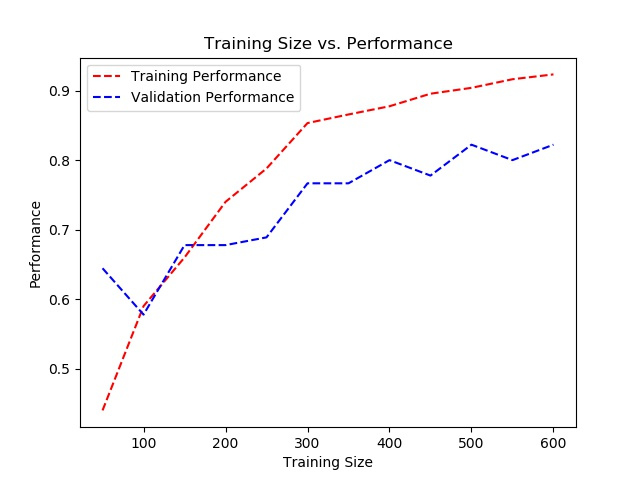
\includegraphics[scale=0.75, width=\linewidth]{Trainsize.jpg}
\caption{Graph comparing size of training set size vs. training accuracy and validation in increments of 50 images}
\label{fig:Trainsize}
\end{figure}
\end{center}
A potential explanation for the results in the figure may be that the training and validation sets, when split amongst the individual actors, may be favouring some actors over others.  There is an intersection at 100 training examples, and it appears the the accuracy between the two sets is almost identical.  The fact that there is a large discrepancy between the accuracies between a training sample size of ~180 to ~300 (e.g. validation accuracy stays relatively constant) may reveal support for the above claim that actors are not being represented properly, presumably due to a lack of rigour in the splitting between data sets for the individual actors.  Upon testing on the other actors and actresses not included in $act$, the validation accuracy obtained was $69\%$.  As outlined in the \textbf{Post-Mortem Addendum} in Section 2, the selection of data from the images may also have played a role in this behaviour.

\end{homeworkProblem}
\clearpage
%----------------------------------------------------------------------------------------
%----------------------------------------------------------------------------------------
%	PROBLEM 6
%----------------------------------------------------------------------------------------

\begin{homeworkProblem}
\noindent \textit{Mathematical Derivations of Gradient Descent}
\begin{enumerate}[label=(\Alph*)]
\item We can compute $\frac{\partial J}{\partial \theta_{pq}}$ by expanding the expression as outlined in the assignment documentation as follows:
\begin{center}
$J(\theta)=\sum_{i}\big((\theta^Tx^{(i)}-y^{(i)})^2_1+(\theta^Tx^{(i)}-y^{(i)})^2_2+\ldots+(\theta^Tx^{(i)}-y^{(i)})^1_j\big)$
\linebreak
$J(\theta)=(\theta^Tx^{(1)}-y^{(1)})^2_1+(\theta^Tx^{(1)}-y^{(1)})^2_2+\ldots(\theta^Tx^{(1)}-y^{(1)})^1_j+(\theta^Tx^{(2)}-y^{2)})^2_1+\ldots + (\theta^Tx^{(i)}-y^{(i)})^2_j$
\end{center}
Therefore, it appears we can model this double summation as a summation over the $p^{th}$ column and $q^{th}$ row.  Therefore, the partial derivative of a specific element, say, element $pq$ can be expressed as:
\begin{center}
$\boxed{\frac{\partial J}{\partial \theta _{pq}}=2x^{p}_{q}(\theta^T x^{p}-y^{p})_q}$
\end{center}
\item Based on the assignment specification, let $X$ be a matrix of size $n \times m$, where $n$ is the number of features and $m$ is the number of training examples.  Let $\theta$ be a matrix of size $k \times n$, where $k$ is the number of features.  Let $Y$ be a $k \times m$ matrix.  The provided expression taken from the assignment specification, with matrices substituted into their respective variables, gives the following expression:
\[2\begin{bmatrix}
x_{11} & \dots & x_{1m} \\
\vdots & \ddots & \vdots \\
x_{n1} & \dots & x_{nk}
\end{bmatrix}\times
\Bigg[\begin{bmatrix}
\theta_{11} & \dots & \theta_{1n} \\
\vdots & \ddots & \vdots \\
\theta_{k1} & \dots & \theta_{kn}
\end{bmatrix}^T \times
\begin{bmatrix}
x_{11} & \dots & x_{1m} \\
\vdots & \ddots & \vdots \\
x_{n1} & \dots & x_{nm}
\end{bmatrix} - 
\begin{bmatrix}
y_{11} & \dots & y_{1m} \\
\vdots & \ddots & \vdots \\
y_{k1} & \dots & y_{km}
\end{bmatrix}\Bigg]^T
\]

Simplification:
\[\begin{bmatrix}
2x_{11} & \dots & 2x_{1m} \\
\vdots & \ddots & \vdots \\
2x_{n1} & \dots & 2x_{nk}
\end{bmatrix}\times
\begin{bmatrix}
\theta_{11}x_{11}+\ldots +  \theta_{k1}x_{n1}-y_{11} & \dots \\
\vdots & \vdots  \\
\dots  & \theta_{1n}x_{1m}+\ldots+\theta_{kn}x_{nm}-y_{km}
\end{bmatrix}^T
\]
If the above matrix computation is carried out, we can observe, from part A, that the $pq$ term in the derivative of the cost function refers to an element within this gradient matrix.  For example, the top left hand side derivative, e.g. $\frac{\partial J}{\partial \theta_{11}}=2x_{11}(\theta_{11}x_{11}+\ldots + \theta_{k1}x_{n1}-y_{11}$.
\textbf{Note:}  The top left hand corner element of the gradient was selected for ease of computation, but any element within this gradient matrix would be valid.
\begin{lstlisting}
#Cost Function
def f2(x,y,theta):
    ones = np.ones((1,x.shape[1]))
    x = np.vstack((ones,x))
    hypothesis = np.matmul(theta.T,x)
    loss = np.power((hypothesis-y),2)
    return np.sum(loss)
\end{lstlisting}
\begin{lstlisting}
#Gradient Function
def df2(x,y,theta):
    ones = np.ones((1,x.shape[1]))
    x = vstack((ones,x))
    hypothesis = np.matmul(np.transpose(theta),x)-y
    hypothesis = np.transpose(hypothesis)
    gradient = 2*np.matmul(x,hypothesis)
    return gradient
\end{lstlisting}
\item The code for testing the implementation of the cost and gradient is shown below.
\begin{lstlisting}
#Testing the cost and gradient functionality
def part6():
    #Testing the loss function
    x = np.random.normal(0,0.6,(20,15))
    y = np.random.normal(0.2,0.4,(5,15))
    theta = np.random.normal(-0.1,0.3,(21,5))
    h = 0.00001
    #Cost of individual component
    testarr1 = np.zeros(theta.shape)
    testarr1[3,4] = h
    print("Cost is:")
    print((f2(x,y,theta+testarr1)-f2(x,y,theta-testarr1))/(2*h))
    print("Gradient is:")
    print(df2(x,y,theta)[3,4])
    testarr2 = np.zeros(theta.shape)
    testarr2[1,4] = h
    print("Cost is:")
    print((f2(x,y,theta+testarr2)-f2(x,y,theta-testarr2))/(2*h))
    print("Gradient is:")
    print(df2(x,y,theta)[1,4])
    testarr3 = np.zeros(theta.shape)
    testarr3[2,3] = h
    print("Cost is:")
    print((f2(x,y,theta+testarr3)-f2(x,y,theta-testarr3))/(2*h))
    print("Gradient is:")
    print(df2(x,y,theta)[2,3])
    testarr4 = np.zeros(theta.shape)
    testarr4[8,4] = h
    print("Cost is:")
    print((f2(x,y,theta+testarr4)-f2(x,y,theta-testarr4))/(2*h))
    print("Gradient is:")
    print(df2(x,y,theta)[8,4])
    testarr5 = np.zeros(theta.shape)
    testarr5[10,1] = h
    print("Cost is:")
    print((f2(x,y,theta+testarr5)-f2(x,y,theta-testarr5))/(2*h))
    print("Gradient is:")
    print(df2(x,y,theta)[10,1])
\end{lstlisting}
The output that results from execution of this code is below:
\begin{lstlisting}
Cost is:
-8.507892229658864
Gradient is:
-8.5078922306346
Cost is:
-5.070817460506305
Gradient is:
-5.070817460432679
Cost is:
-11.655092452400593
Gradient is:
-11.655092451975934
Cost is:
-3.5024079892309596
Gradient is:
-3.5024079896724483
Cost is:
-0.24353752436923057
Gradient is:
-0.2435375237734189
\end{lstlisting}
The $h$ was selected so as to try to compute a small difference, similar to the definition of the derivative - as $h$ further decreases, you would observe that the gradient and incremental difference in cost appear to converge.
\end{enumerate}

\end{homeworkProblem}
\clearpage
%----------------------------------------------------------------------------------------
%	PROBLEM 7
%----------------------------------------------------------------------------------------

\begin{homeworkProblem}

\noindent \textit{Linear Regression with Multiple Actors}

Running the linear regression classifier results in a training accuracy of $89\%$ and a validation accuracy of $56\%$.  Both the $\alpha$ and number of iterations were modified, to varying degrees of success - however, it is worth noting that the validation accuracy is significantly lower than the training accuracy which may be a symptom of overfitting.
\par Two loops were written in order to obtain the training hypothesis and validation hypothesis labels.  The steps are written below.
\begin{enumerate}
\item A matrix of 0's was initialized to the same shape as that of the label matrix
\item Each column in the label matrix was scanned for it's maximum value and the index of that value was stored in a new variable, \textit{max}
\item Starting at the $0^{th}$ column, a 1 was stored into the 0's matrix for each index in \textit{max}, and iterated through until the last column was reached.
\item The resultant matrix now had only one value of 1 in each column and was compared to the label matrix.
\end{enumerate}
An example of this for the training data is shown below.
\begin{lstlisting}
    #Training hypothesis
    ones_t = np.ones((1,training.shape[1]))
    training_with_bias = vstack((ones_t,training))
    training_hypothesis = np.matmul(theta.T,training_with_bias)
    max = training_hypothesis.argmax(axis=0)
    max = np.array(max)
    training_hypothesis_labels = np.zeros((training_hypothesis.shape))
    print(training_hypothesis_labels.shape)
    i = 0
    while i < training_hypothesis_labels.shape[1]:
        index = max[i]
        training_hypothesis_labels[index,i]=1
        i+=1

    correct = 0
    i = 0
    while i < training_hypothesis_labels.shape[1]:
        if np.array_equal(training_hypothesis_labels[:,i],training_labels[:,i]) is True:
            correct += 1
        i+=1
    print("Training accuracy is: " + str(correct/600.0))

\end{lstlisting}

\end{homeworkProblem}
\clearpage
%----------------------------------------------------------------------------------------
%	PROBLEM 8
%----------------------------------------------------------------------------------------
\begin{homeworkProblem}
\noindent \textit{Visualizing $\theta 's$ with multiple label matrix}

The 6 figures below show the visualized $\theta 's$ for training on the full set of actors in $act$ with the label matrix, as outlined in the assignment specification.
\begin{center}
\begin{figure}[!ht]\centering
\begin{subfigure}{.3\textwidth}\centering
  
\includegraphics[width=.3\linewidth]{thetas0.jpg}
  \caption{Baldwin $\theta 's$}
\end{subfigure}
\begin{subfigure}{.3\textwidth}\centering
  
\includegraphics[width=.3\linewidth]{thetas1.jpg}
  \caption{Bracco $\theta 's$}
\end{subfigure}
\begin{subfigure}{.3\textwidth}\centering
  
\includegraphics[width=.3\linewidth]{thetas2.jpg}
  \caption{Carell $\theta 's$}
\end{subfigure}
\begin{subfigure}{.3\textwidth}\centering
  
\includegraphics[width=.3\linewidth]{thetas3.jpg}
  \caption{Gilpin $\theta 's$}
\end{subfigure}
\begin{subfigure}{.3\textwidth}\centering
  
\includegraphics[width=.3\linewidth]{thetas4.jpg}
  \caption{Hader $\theta 's$}
\end{subfigure}
\begin{subfigure}{.3\textwidth}\centering
  
\includegraphics[width=.3\linewidth]{thetas5.jpg}
  \caption{Harmon $\theta 's$}
\end{subfigure}
\caption{$\theta$ values for each individual actor}
\end{figure}
\end{center}
A potential explanation for the lack of "face-like" appearance in $\theta 's $ obtained after training may be that the size of the training set is too large for each actor.  As observed in part 4, with only two actors from the Baldwin and Carell sets, the $\theta 's$ visualized more resembled faces.
\end{homeworkProblem}
\end{document}